\documentclass[conference]{IEEEtran}

% --- Packages ---
\usepackage{graphicx}
\usepackage{amsmath}
\usepackage{amssymb,amsfonts}
\usepackage{mathtools}
\usepackage{array}
\usepackage{cite}
\usepackage{booktabs}
\usepackage{float}

% --- Custom operators ---
\DeclareMathOperator*{\argmax}{arg\,max}
\newcommand{\E}{\mathbb{E}}

% --- Title & Author ---
\title{Intelligent Traffic Signal Control using Reinforcement Learning: \\ 
A Comparative Study of Fixed-Time, LQF, Q-Learning, and DQN}

\author{
    Yashwanth Balamurugan \\ 
    Department of Computer Science \\ 
    National Institute of Technology, Warangal \\ 
    Email: your.email@example.com
}

\begin{document}
\maketitle

% --- Abstract ---
\begin{abstract}
Traffic congestion is a critical challenge in modern cities. Conventional controllers, such as fixed-time scheduling, fail to adapt to fluctuations in demand, leading to long waiting times and wasted energy. In this work, we study a single four-way intersection and evaluate four control strategies: Fixed-Time, Longest Queue First (LQF), Q-Learning, and Deep Q-Network (DQN). The system integrates SUMO with Python via TraCI, and performance is measured using cumulative average waiting time. Results show that learning-based controllers significantly outperform traditional approaches. Surprisingly, Q-Learning achieved the lowest average waiting time of 16.72 s, outperforming the more complex DQN (20.66 s). This highlights that for small-scale intersections, well-engineered state discretization may outperform deep models.
\end{abstract}

% --- Introduction ---
\section{Introduction}
Urban traffic congestion results in increased travel times, higher fuel consumption, and pollution. Traditional fixed-time controllers are widely deployed but lack adaptiveness to dynamic and stochastic traffic flows.  

Recent advances in Reinforcement Learning (RL) have enabled traffic light controllers that learn adaptive policies through interaction with their environment. While Deep Reinforcement Learning (DRL) approaches such as Deep Q-Networks (DQN) have shown success in large-scale traffic control \cite{mnih2015,wei2018}, simpler approaches like tabular Q-Learning may still be effective in small, structured scenarios.  

In this paper, we evaluate four controllers for a single isolated intersection: Fixed-Time, Longest Queue First (LQF), Q-Learning, and DQN. We simulate realistic traffic in SUMO and analyze comparative performance.

% --- Related Work ---
\section{Related Work}
Conventional signal control methods include Webster’s formula and Max-pressure control, which optimize based on static or heuristic rules. While effective in predictable conditions, these methods fail under high variability.  

Reinforcement Learning has emerged as a strong alternative. Early works applied tabular Q-learning to single intersections \cite{sutton2018}, while more recent studies use DQN and policy gradient methods to scale to larger networks \cite{liang2019,wei2018}. Actor-critic algorithms such as DDPG have also been proposed for continuous action spaces.  

Multi-Agent Reinforcement Learning (MARL) is another direction, where each intersection is modeled as an agent, and coordination emerges across the network. However, scalability and convergence remain open challenges.  

This project focuses on the single-intersection scenario, serving as a baseline before extending to multi-agent systems.

% --- System Model ---
\section{System Model and Problem Formulation}
We model the traffic signal control as a Markov Decision Process (MDP):
\[
\mathcal{M} = (\mathcal{S}, \mathcal{A}, P, R, \gamma)
\]
where:
\begin{itemize}
    \item $\mathcal{S}$: state space, defined by queue lengths and waiting times of all lanes,
    \item $\mathcal{A}$: set of actions (phases to activate),
    \item $P$: transition probabilities of traffic flow,
    \item $R$: reward function based on vehicle waiting time,
    \item $\gamma$: discount factor.
\end{itemize}

\textbf{State:} Normalized queue lengths for each direction.  
\textbf{Action:} Selecting one of the four phases (North, East, South, West).  
\textbf{Reward:} 
\[
r_t = - \sum_{i=1}^{n} W_i(t)
\]
where $W_i(t)$ is the waiting time of vehicles in lane $i$ at time $t$.  

Objective:
\[
\pi^* = \argmax_\pi \E \left[ \sum_{t=0}^\infty \gamma^t r_t \right]
\]

% --- Network Diagram ---
\begin{figure}[H]
    \centering
    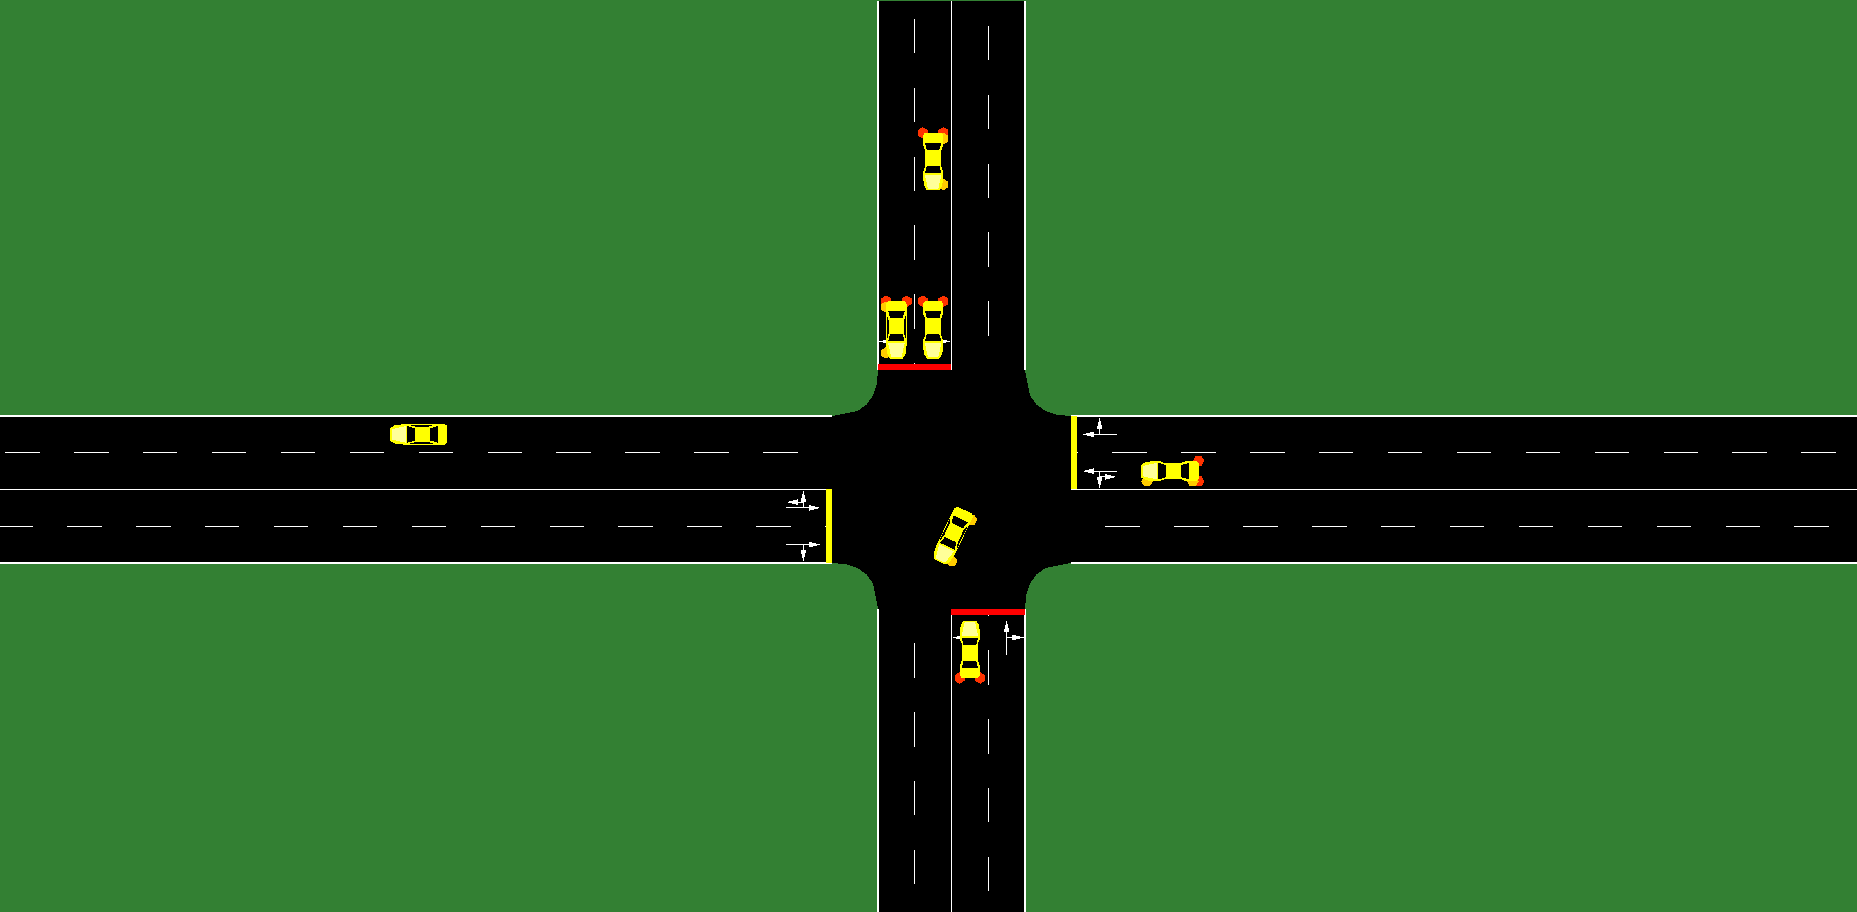
\includegraphics[width=0.8\columnwidth]{intersection_network.png}
    \caption{Single Intersection Network used in simulations.}
    \label{fig:intersection_network}
\end{figure}

% --- Methodology ---
\section{Methodology}
\subsection{Fixed-Time Controller}
Cycle length:
\[
C = \sum_{i=1}^{n} g_i + \sum_{i=1}^{n} y_i
\]
with fixed $g_i, y_i$. Best suited for stable, predictable flows.

\subsection{Longest Queue First (LQF)}
Rule-based:
\[
a^* = \argmax_{i \in \mathcal{A}} Q_i
\]
where $Q_i$ is the current queue length. Effective for imbalanced traffic but may starve low-demand lanes.

\subsection{Q-Learning}
Update rule:
\[
Q(s,a) \leftarrow Q(s,a) + \alpha \big[ r + \gamma \max_{a'} Q(s',a') - Q(s,a) \big]
\]
with discretized states (\emph{low, medium, high} queue levels). Effective for small discrete spaces.

\subsection{Deep Q-Network (DQN)}
Neural approximation $Q(s,a;\theta)$. Loss:
\[
L(\theta) = \E_{(s,a,r,s') \sim \mathcal{D}} 
\Big[ \big( r + \gamma \max_{a'} Q(s',a';\theta^-) - Q(s,a;\theta) \big)^2 \Big]
\]

Exploration via $\epsilon$-greedy policy. Handles continuous states but requires careful tuning.

% --- Simulation Setup ---
\section{Simulation Setup}
We implemented the system in SUMO with TraCI as the interface.  

\textbf{Intersection:} Single four-way junction with two lanes per approach.  
\textbf{Traffic flow:} Randomized vehicle arrivals using SUMO \texttt{<flow>} definitions.  
\textbf{Simulation length:} 3600 steps (1 simulated hour).  
\textbf{Controllers:} Fixed-Time, LQF, Q-Learning, DQN.  
\textbf{Metric:} Cumulative Average Vehicle Waiting Time:
\[
W_{avg}(t) = \frac{1}{N(t)} \sum_{i=1}^{N(t)} w_i(t)
\]

% --- Results ---
\section{Results and Discussion}
The final performance after 3600 steps is summarized in Table~\ref{tab:results}. Trends are shown in Fig.~\ref{fig:plot}.

\begin{table}[H]
    \centering
    \caption{Final Average Wait Times after 3600 Steps}
    \label{tab:results}
    \begin{tabular}{lc}
        \toprule
        \textbf{Controller} & \textbf{Final Avg Wait Time (s)} \\
        \midrule
        Fixed-Time & 54.72 \\
        LQF & 34.37 \\
        DQN & 20.66 \\
        \textbf{Q-Learning} & \textbf{16.72} \\
        \bottomrule
    \end{tabular}
\end{table}

\begin{figure}[H]
    \centering
    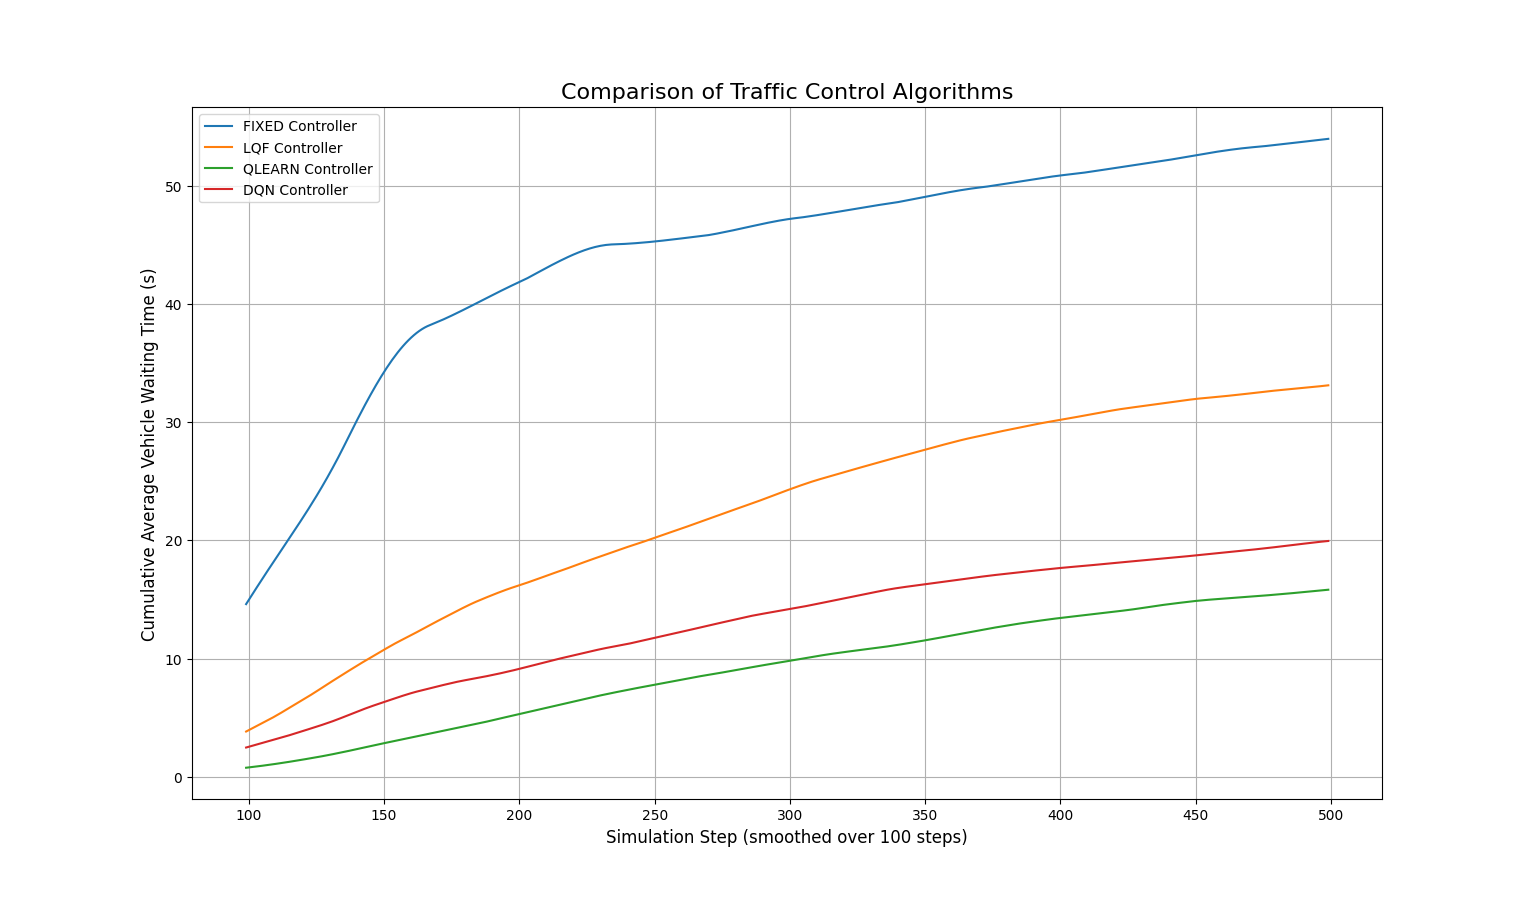
\includegraphics[width=\columnwidth]{comparison_plot.png}
    \caption{Cumulative average waiting time comparison across controllers.}
    \label{fig:plot}
\end{figure}

\textbf{Findings:}
\begin{itemize}
    \item \textbf{Fixed-Time:} Performed worst due to rigidity.  
    \item \textbf{LQF:} Reactive but shortsighted.  
    \item \textbf{DQN:} Achieved low waiting times, but sensitive to tuning.  
    \item \textbf{Q-Learning:} Outperformed DQN. Discretized states provided strong feature engineering, leading to fast convergence and stability.  
\end{itemize}

% --- DDPG & Future Work ---
\section{Consideration of DDPG and Future Work}
An initial experiment was conducted with the Deep Deterministic Policy Gradient (DDPG) algorithm, another prominent DRL method. However, the DDPG agent failed to converge and resulted in extremely high waiting times, showing it was unsuitable for this problem.  

DDPG is an actor-critic method designed for \textbf{continuous action spaces}. Our problem involves a \textbf{discrete action space} (four phases), making DDPG unstable and inefficient. Value-based methods (Q-Learning, DQN) are more appropriate here.  

\subsection{Future Work: Grid Networks}
The true strength of DDPG lies in large, complex problems such as \textbf{multi-intersection grid control}. In such settings, the joint action space grows exponentially, making DQN infeasible. Actor-critic methods like DDPG can directly learn policies in vast action spaces, enabling coordination across intersections.  

\begin{figure}[H]
    \centering
    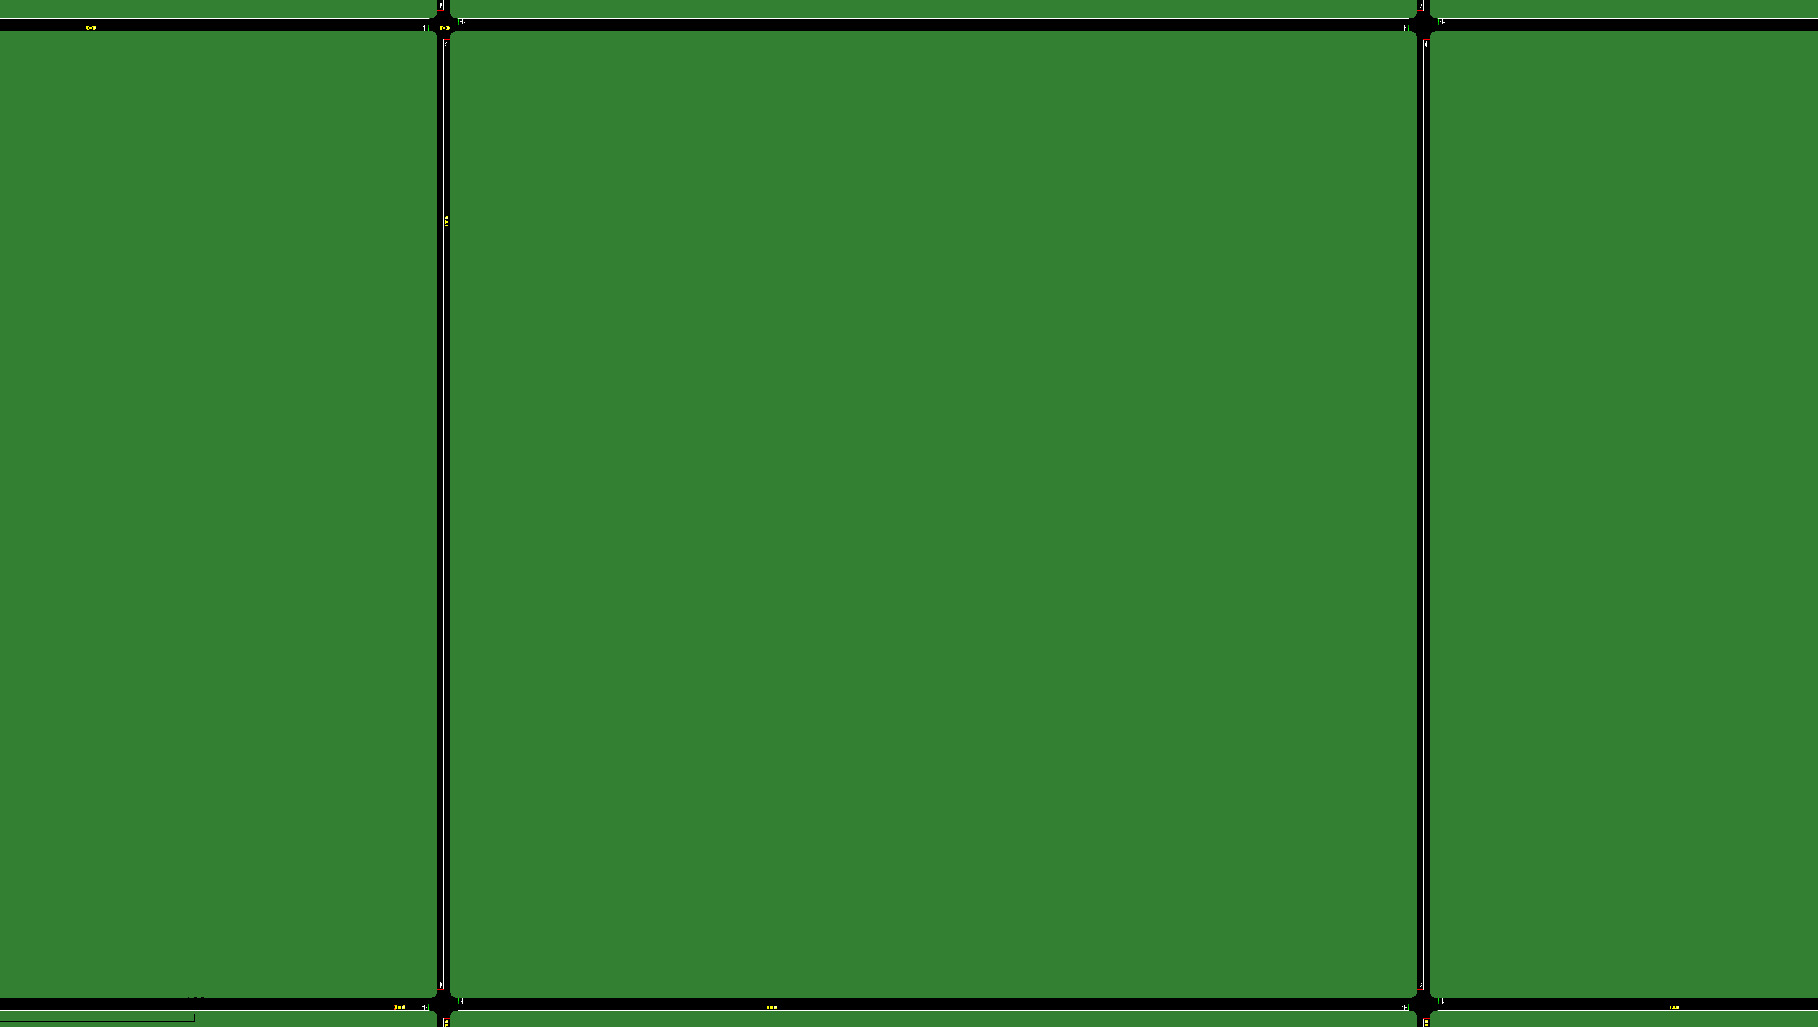
\includegraphics[width=0.8\columnwidth]{grid_network.png}
    \caption{Example of a Multi-Intersection Grid Network for future work.}
    \label{fig:grid_network}
\end{figure}

Future research should extend this work to grid networks, investigating centralized or multi-agent DDPG for emergent behaviors like the ``greenwave'' effect \cite{zhu2025deep}.

% --- Conclusion ---
\section{Conclusion}
This study compared four traffic light controllers. Results show that reinforcement learning, particularly Q-Learning with discretized states, significantly outperforms traditional methods. Surprisingly, Q-Learning also outperformed DQN in this scenario, highlighting the role of state representation.  

Future work includes extending to multi-intersection grids and exploring Multi-Agent RL with actor-critic agents like DDPG for large-scale coordination.

% --- References ---
\bibliographystyle{IEEEtran}
\begin{thebibliography}{00}

\bibitem{mnih2015}
V. Mnih et al., ``Human-level control through deep reinforcement learning,'' \textit{Nature}, vol. 518, pp. 529--533, 2015.

\bibitem{sutton2018}
R. S. Sutton and A. G. Barto, \textit{Reinforcement Learning: An Introduction}, 2nd ed. MIT Press, 2018.

\bibitem{wei2018}
H. Wei, G. Zheng, H. Yao, and Z. Li, ``Intellilight: A reinforcement learning approach for intelligent traffic light control,'' in \textit{ACM SIGKDD}, pp. 2496--2505, 2018.

\bibitem{liang2019}
X. Liang, X. Du, G. Wang, and Z. Han, ``A deep reinforcement learning network for traffic light cycle control,'' \textit{IEEE Trans. Vehicular Tech.}, vol. 68, no. 2, pp. 1243--1253, 2019.

\bibitem{zhu2025deep}
M. Zhu, X.-Y. Liu, S. Borst, and A. Walid, ``Deep Reinforcement Learning for Traffic Light Control in Intelligent Transportation Systems,'' \textit{IEEE Trans. Netw. Sci. Eng.}, vol. XX, 2025.

\end{thebibliography}

\end{document}
